\section{Object Detection Using Exemplar Models} % (fold)
\label{cha:object_detection}

\todo[inline]{Write short introduction, making the bridge between related work and Exemplar models}

\subsection{Exemplar Models} % (fold)
\label{sub:exemplar_models}

Exemplar models are related to part-based models.\cite{leibe2004combined, chum2007exemplar} Exemplar models do not explicitly model object parts, but they do something similar implicitly on the feature level. In this approach, for each object feature found during training, an exemplar is stored. The exemplar represents the size and location of the bounding box relative to the feature. The exemplars are aggregated into part models\cite{leibe2004combined} or visual words\cite{chum2007exemplar}. In this way a class is modeled by a set of exemplars that have a high probability of occurring in a certain location and at a certain scale of the image.

At test time, each feature found in the test image is matched with the exemplars stored, and from this combination of the location and scale of the feature found, and the exemplar it is matched with, a hypothesis can be formed for the object's location in the test image. This means that each feature in the test image gets a vote, weighted by the quality of its match, for a bounding box. These hypotheses can be clustered into detection windows. Experiments\cite{vedaldi2009multiple} show that this method performs well too as a first step in a cascade setting.

In more detail, 

\todo[inline,color=green]{part on why I choose exemplar models, little more explanation of theory of Chum to link it to the next section}
% subsection exemplar_models (end)

\subsection{Clustering Algorithms} % (fold)
\label{sub:clustering_algorithms}

Clustering is a way to find classes of items without having a predefined idea of what these classes represent. It is a form of unsupervised learning, meaning that there are no ground-truth classes available. Usually the parameters of the classes are unknown, and often also the number of classes is not predefined. Clustering algorithms can be applied to all all kinds of situations.

In exemplar-model detection, hypotheses of bounding boxes need to be clustered into detections. These detections represent the classes, which are inherently unknown, and depend fully on the image at hand, and the hypotheses that have been derived from it. The number of objects in the image is unknown, so the number of clusters should not be fixed.

A number of algorithms exist that can be used to cluster objects. A well known algorithm is called k-means clustering. This algorithm divides all objects in a pre-defined number of $k$ clusters, minimizing the sum of squared distances of all objects within each separate cluster. This is calculated iteratively by assigning each object to the cluster with the nearest cluster center, and then setting the cluster's center at the mean position of all its members. One important downside of this algorithm for the detection problem is that we do not have an indication of the number of clusters wanted. Therefore, other algorithms can be considered.

\begin{figure}[hbt]
    \label{fig:sl_vs_qs_clustering}
    \centering
    \missingfigure[figwidth=0.8\textwidth]{Single Link clustering vs Quickshift clustering.}
\end{figure}

\todo[inline]{Include an image comparing the clustering algorithms mentioned: see diff between aggl. clustering and quickshift}

\subsubsection{Agglomerative Clustering} % (fold)
\label{sub:agglomerative_clustering}
It is possible to view a clustering clustering algorithm as a tree, where the leaves represent the objects to be clustered. If the pairwise distances between all objects are known, the leaves can be joined into clusters iteratively, each time merging the two closest objects into a cluster. When these clusters are again clustered based on distance, merging will continue until there is only one single cluster left. Afterwards, this tree could be split into clusters by cutting branches that exceed a certain threshold distance. This clustering algorithm is called Agglomerative clustering. It is a subtype of hierarchical clustering, other hierarchical algorithms not being agglomerative, but divisive, starting with one single cluster.

There is some variety in the ways to merge leaves into clusters. Single link clustering means that the minimum distance between members of each cluster is the basis of further clustering, complete linkage and mean linkage clustering take the maximum distance and the mean distance, respectively.

\todo[inline]{More explanation and some image}

% subsubsection agglomerative_clustering (end)

\subsubsection{Mode-seeking Algorithms} % (fold)
\label{sub:mode_finding_algorithms}
\todo[inline]{mean-shift,Quickshift, difference with hierarchical clustering, benefits, image}

Finding local maxima of a density function (pdf) = mode-seeking.
Mean-shift clustering finds these local maxima and assigns the data points to it (sort of gradient ascent)

\begin{figure}[hbt]
    \centering
    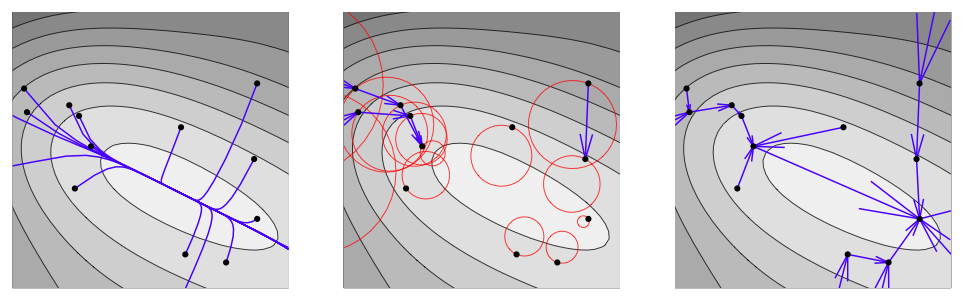
\includegraphics[width=0.8\textwidth]{MeanshiftMedianshiftQuickshift}
    \caption{Mean shift clustering (left) vs. Median Shift clustering (center) vs. Quickshift clustering (right)}
    \label{fig:meanshift_median_shift_quickshift}
\end{figure}

% subsubsection mode_finding_algorithms (end)

% subsection clustering_algorithms (end)

% section object_detection (end)
